\documentclass[12pt]{ctexart}
\usepackage[a4paper,margin=1in]{geometry}
\usepackage{amsmath,amssymb,siunitx,booktabs,multirow,gensymb}
\usepackage{graphicx}
\usepackage{tikz}
\usetikzlibrary{arrows.meta,positioning,calc,shapes.geometric,shadows}
\usepackage{algorithm}
\usepackage{algpseudocode}
\floatname{algorithm}{算法}
\renewcommand{\algorithmicrequire}{\textbf{输入:}}
\renewcommand{\algorithmicensure}{\textbf{输出:}}

% --- 代码美化 ---
\usepackage[most]{tcolorbox}
\usepackage{xcolor}
\usepackage{listings}
\tcbuselibrary{listings}

% 定义Python语法高亮颜色
\definecolor{pyblue}{RGB}{0,102,204}
\definecolor{pygreen}{RGB}{0,128,0}
\definecolor{pyred}{RGB}{204,0,0}
\definecolor{pyorange}{RGB}{255,140,0}
\definecolor{pygray}{RGB}{128,128,128}
\definecolor{pypurple}{RGB}{128,0,128}
\definecolor{pycyan}{RGB}{0,128,128}
\definecolor{pybg}{RGB}{248,248,248}

% 定义C++语法高亮颜色
\definecolor{cppblue}{RGB}{0,0,255}
\definecolor{cppgreen}{RGB}{0,128,0}
\definecolor{cppred}{RGB}{163,21,21}
\definecolor{cpporange}{RGB}{255,165,0}
\definecolor{cppgray}{RGB}{128,128,128}
\definecolor{cpppurple}{RGB}{128,0,128}
\definecolor{cppbg}{RGB}{248,248,255}

% Python语言定义
\lstdefinelanguage{Python3}{
  language=Python,
  morekeywords={and,as,assert,break,class,continue,def,del,elif,else,except,
    False,finally,for,from,global,if,import,in,is,lambda,None,nonlocal,not,
    or,pass,raise,return,True,try,while,with,yield,async,await,self},
  sensitive=true,
  morecomment=[l]{\#},
  morecomment=[s]{"""}{"""},
  morecomment=[s]{'''}{'''},
  morestring=[b]',
  morestring=[b]",
  morestring=[b]',
  morestring=[b]",
  alsoletter={_},
  alsoother={\$},
  moredelim=[is][\color{pyorange}]{@}{@},
}

% C++语言定义增强
\lstdefinestyle{C++Enhanced}{
  language=C++,
  morekeywords={auto,constexpr,decltype,nullptr,override,final,
    noexcept,static_assert,thread_local,unique_ptr,shared_ptr,weak_ptr,
    make_unique,make_shared,const_cast,static_cast,dynamic_cast,
    reinterpret_cast,sizeof,alignof,alignas,decltype},
  moredirectives={\#include,\#define,\#ifdef,\#ifndef,\#endif,\#pragma},
  sensitive=true,
  morecomment=[l]{//},
  morecomment=[s]{/*}{*/},
  morestring=[b]",
  morestring=[b]',
  alsoletter={_},
  alsoother={\$,\&,\*,\->,::,&&,||,==,!=,<=,>=,<,>,+,-,/,\%,~,^,|,\&},
}

\newtcblisting{pythoncode}[1][]{
  enhanced,
  colback=pybg,
  colframe=pyblue!70!black,
  listing only,
  listing options={
    language=Python3,
    basicstyle=\ttfamily\footnotesize,
    keywordstyle=\color{pyblue}\bfseries,
    stringstyle=\color{pyred},
    commentstyle=\color{pygreen}\itshape,
    numbers=left,
    numberstyle=\tiny\color{pygray}\ttfamily,
    numbersep=8pt,
    breaklines=true,
    breakatwhitespace=true,
    tabsize=4,
    showstringspaces=false,
    frame=single,
    frameround=tttt,
    framesep=5pt,
    backgroundcolor=\color{pybg},
    xleftmargin=15pt,
    xrightmargin=5pt,
    aboveskip=10pt,
    belowskip=10pt,
    captionpos=b,
    emph={self,True,False,None},
    emphstyle=\color{cpppurple}\bfseries
  },
  title={\textbf{Python 代码}: #1},
  fonttitle=\bfseries\small,
  coltitle=white,
  colbacktitle=pyblue,
  sharp corners,
  drop shadow={shadow scale=1.1, shadow xshift=1pt, shadow yshift=-1pt},
  boxrule=0.5pt,
  arc=2pt,
  outer arc=2pt,
  attach boxed title to top left={yshift=-2mm,xshift=2mm}
}

% 简化的inline代码样式
\newtcblisting{pythoninline}[1][]{
  enhanced,
  colback=pybg,
  colframe=pyblue!50!black,
  listing only,
  listing options={
    language=Python3,
    basicstyle=\ttfamily\scriptsize,
    keywordstyle=\color{pyblue},
    stringstyle=\color{pyred},
    commentstyle=\color{pygreen}\itshape,
    numbers=none,
    breaklines=true,
    tabsize=2,
    showstringspaces=false
  },
  arc=1mm,
  boxrule=0.3pt,
  left=2pt,right=2pt,top=1pt,bottom=1pt,
  #1
}

% 用于高亮特定行的Python代码
\newtcblisting{pythonhighlight}[2][]{
  enhanced,
  colback=pybg,
  colframe=pyblue!70!black,
  listing only,
  listing options={
    language=Python3,
    basicstyle=\ttfamily\footnotesize,
    keywordstyle=\color{pyblue}\bfseries,
    stringstyle=\color{pyred},
    commentstyle=\color{pygreen}\itshape,
    numbers=left,
    numberstyle=\tiny\color{pygray}\ttfamily,
    numbersep=8pt,
    breaklines=true,
    tabsize=4,
    showstringspaces=false,
    emphstyle={\color{pyorange}\bfseries\underbar},
    moreemph={#2}
  },
  title={\textbf{Python 代码}: #1},
  fonttitle=\bfseries\small,
  coltitle=white,
  colbacktitle=pyblue,
  sharp corners,
  drop shadow={shadow scale=1.1, shadow xshift=1pt, shadow yshift=-1pt},
  boxrule=0.5pt,
  arc=2pt,
  outer arc=2pt
}

\newtcblisting{cppcode}[1][]{
  enhanced,
  colback=cppbg,
  colframe=cppblue!70!black,
  listing only,
  listing options={
    style=C++Enhanced,
    basicstyle=\ttfamily\footnotesize,
    keywordstyle=\color{cppblue}\bfseries,
    stringstyle=\color{cppred},
    commentstyle=\color{cppgreen}\itshape,
    numbers=left,
    numberstyle=\tiny\color{cppgray}\ttfamily,
    numbersep=8pt,
    breaklines=true,
    breakatwhitespace=true,
    tabsize=4,
    showstringspaces=false,
    frame=single,
    frameround=tttt,
    framesep=5pt,
    backgroundcolor=\color{cppbg},
    xleftmargin=15pt,
    xrightmargin=5pt,
    aboveskip=10pt,
    belowskip=10pt,
    captionpos=b,
    emph={Index,Real,Vector3,Matrix3D,NodeGenericData,ObjectContactFewTeeth,
           ObjectContactCircleCircle,ObjectContactCurveCircles,
           MarkerBodyRigid,SimulationSettings,DynamicSolverType,
           PostNewtonFlags,GeneralizedAlpha},
    emphstyle=\color{cpppurple}\bfseries
  },
  title={\textbf{C++ 代码}: #1},
  fonttitle=\bfseries\small,
  coltitle=white,
  colbacktitle=cppblue,
  sharp corners,
  drop shadow={shadow scale=1.1, shadow xshift=1pt, shadow yshift=-1pt},
  boxrule=0.5pt,
  arc=2pt,
  outer arc=2pt,
  attach boxed title to top left={yshift=-2mm,xshift=2mm}
}

% 简化的inline C++代码样式
\newtcblisting{cppinline}[1][]{
  enhanced,
  colback=cppbg,
  colframe=cppblue!50!black,
  listing only,
  listing options={
    style=C++Enhanced,
    basicstyle=\ttfamily\scriptsize,
    keywordstyle=\color{cppblue},
    stringstyle=\color{cppred},
    commentstyle=\color{cppgreen}\itshape,
    numbers=none,
    breaklines=true,
    tabsize=2,
    showstringspaces=false
  },
  arc=1mm,
  boxrule=0.3pt,
  left=2pt,right=2pt,top=1pt,bottom=1pt,
  #1
}

% 用于高亮特定行的C++代码
\newtcblisting{cpphighlight}[2][]{
  enhanced,
  colback=cppbg,
  colframe=cppblue!70!black,
  listing only,
  listing options={
    style=C++Enhanced,
    basicstyle=\ttfamily\footnotesize,
    keywordstyle=\color{cppblue}\bfseries,
    stringstyle=\color{cppred},
    commentstyle=\color{cppgreen}\itshape,
    numbers=left,
    numberstyle=\tiny\color{cppgray}\ttfamily,
    numbersep=8pt,
    breaklines=true,
    tabsize=4,
    showstringspaces=false,
    emphstyle={\color{cpporange}\bfseries\underbar},
    moreemph={#2}
  },
  title={\textbf{C++ 代码}: #1},
  fonttitle=\bfseries\small,
  coltitle=white,
  colbacktitle=cppblue,
  sharp corners,
  drop shadow={shadow scale=1.1, shadow xshift=1pt, shadow yshift=-1pt},
  boxrule=0.5pt,
  arc=2pt,
  outer arc=2pt
}

% 额外的代码高亮环境
\newtcblisting{algorithmcode}[1][]{
  enhanced,
  colback=pybg!90!white,
  colframe=pyblue!50!black,
  listing only,
  listing options={
    language=Python3,
    basicstyle=\ttfamily\footnotesize,
    keywordstyle=\color{pyblue}\bfseries,
    stringstyle=\color{pyred},
    commentstyle=\color{pygreen}\itshape,
    numbers=left,
    numberstyle=\tiny\color{pygray}\ttfamily,
    numbersep=5pt,
    breaklines=true,
    breakatwhitespace=true,
    tabsize=2,
    showstringspaces=false,
    frame=single,
    frameround=tttt,
    framesep=2pt,
    backgroundcolor=\color{pybg!95!white},
    xleftmargin=10pt,
    xrightmargin=5pt,
    aboveskip=8pt,
    belowskip=8pt,
    captionpos=b,
    emph={def,class,if,else,for,while,return,import,from,as,try,except,finally},
    emphstyle={\color{pyblue}\bfseries}
  },
  title={\textbf{算法代码}: #1},
  fonttitle=\bfseries\small,
  coltitle=white,
  colbacktitle=pyblue!70!black,
  sharp corners,
  drop shadow={shadow scale=1.05, shadow xshift=0.5pt, shadow yshift=-0.5pt},
  boxrule=0.4pt,
  arc=1pt,
  outer arc=1pt,
  attach boxed title to top left={yshift=-1mm,xshift=1mm}
}

% 配置代码片段环境
\newtcblisting{configcode}[1][]{
  enhanced,
  colback=pybg!95!white,
  colframe=pyorange!50!black,
  listing only,
  listing options={
    language=Python3,
    basicstyle=\ttfamily\footnotesize,
    keywordstyle=\color{pyorange}\bfseries,
    stringstyle=\color{pyred},
    commentstyle=\color{pygreen}\itshape,
    numbers=left,
    numberstyle=\tiny\color{pygray}\ttfamily,
    numbersep=5pt,
    breaklines=true,
    tabsize=2,
    showstringspaces=false,
    frame=single,
    frameround=tttt,
    framesep=2pt,
    backgroundcolor=\color{pybg!98!white},
    xleftmargin=10pt,
    xrightmargin=5pt,
    aboveskip=8pt,
    belowskip=8pt,
    captionpos=b,
    emph={stiffness,damping,friction,contact,mesh,gear},
    emphstyle={\color{pyorange}\bfseries}
  },
  title={\textbf{参数配置}: #1},
  fonttitle=\bfseries\small,
  coltitle=white,
  colbacktitle=pyorange!70!black,
  sharp corners,
  drop shadow={shadow scale=1.05, shadow xshift=0.5pt, shadow yshift=-0.5pt},
  boxrule=0.4pt,
  arc=1pt,
  outer arc=1pt,
  attach boxed title to top left={yshift=-1mm,xshift=1mm}
}

% --- 链接与引用 ---
\usepackage{hyperref}
\hypersetup{
    colorlinks=true,
    linkcolor=blue!70!black,
    citecolor=green!60!black,
    urlcolor=magenta!70!black,
    pdftitle={RV/少齿差减速器建模},
    pdfauthor={}
}
\usepackage[nameinlink]{cleveref}
\crefname{equation}{公式}{公式}
\crefname{figure}{图}{图}
\crefname{table}{表}{表}
\crefname{algorithm}{算法}{算法}
\crefname{section}{节}{节}

\title{\bfseries RV减速器滞回曲线、扭转刚度与回差特性分析}
\author{}
\date{}

\begin{document}
\maketitle

\begin{abstract}
本文聚焦于RV减速器的滞回曲线特性分析，深入探讨了其扭转刚度与回差（Lost Motion）的理论建模与计算方法。采用自定义接触模型模拟摆线轮与针齿、曲柄与轴承等关键部件的相互作用。通过对滞回曲线的仿真计算，量化了RV减速器的非线性刚度特性与传动回差，分析了不同负载工况下的系统响应。文中详细论述了滞回曲线的生成机理、扭转刚度的非线性演变规律以及回差的测定方法，为RV减速器的性能评估与优化设计提供了理论依据。
\end{abstract}

\tableofcontents
\newpage

\section{研究背景与目标}

\subsection{研究对象}
RV 减速器与少齿差减速器是精密传动领域的核心部件，广泛应用于工业机器人、数控机床、航空航天等高精度场合~\cite{rvdynamic,rvfree}。其传动性能直接影响整机的定位精度、重复精度与动态响应特性。

\textbf{少齿差传动}采用内啮合渐开线齿轮副~\cite{litvin}，外齿轮与内齿圈的齿数差通常为 1$\sim$4 齿，通过偏心机构实现大传动比输出。其特点是结构紧凑、承载能力强、传动平稳。

\textbf{RV 减速器}（旋转矢量减速器）采用两级传动：第一级为渐开线行星齿轮，第二级为摆线针轮~\cite{cycloidmodel,cycloidltca}。摆线轮与针齿壳之间形成多点同时接触，具有高刚度、低回差的优点。

\subsection{研究目标}
本研究的核心目标是建立可重用的 RV/少齿差减速器多体动力学模型，实现以下功能：
\begin{enumerate}
  \item \textbf{振动特性分析}：计算系统固有频率、模态振型与强迫振动响应；
  \item \textbf{传动精度评估}：量化传递误差、回程误差与动态定位精度；
  \item \textbf{啮合刚度计算}：获取时变啮合刚度曲线，分析刚度波动对振动的激励；
  \item \textbf{参数优化支持}：为齿廓修形、间隙补偿、预紧力调节等优化设计提供仿真依据。
\end{enumerate}

\subsection{总体技术路线}
为实现上述目标，本研究采用以下技术路线：

\begin{enumerate}
  \item \textbf{自定义接触模型开发}：针对三类典型接触场景（渐开线内啮合、摆线-针列、圆-圆配合），开发专用罚式接触模型，避免通用有限元方法的计算冗余；
  \item \textbf{解析几何表达}：采用渐开线参数方程直接表达齿廓，无需网格离散，保证几何精度与计算效率；
  \item \textbf{时变刚度建模}：基于 Weber-Banaschek 方法与 Hertz 接触理论~\cite{johnson,litvin}，建立位置相关的单齿刚度模型，实现啮合刚度的实时计算；
  \item \textbf{高效接触搜索}：采用角度预筛选、AABB 包围盒过滤与 Warm-start 活跃集技术，降低接触检测的计算复杂度；
  \item \textbf{数值稳健性处理}：通过阻尼正则化、速度缓冲区与接触子步等技术，保证刚性系统的稳定积分。
\end{enumerate}

罚式接触的基本力学模型为：
\begin{equation}
 f_n = k_c \,\max(0,-g)^{n} + d_c \,\max(0,-\dot g), \qquad
 \|f_t\| \le \mu \, f_n ,
 \label{eq:penalty_contact}
\end{equation}
其中 $g$ 为有符号间隙（负值表示穿透），$k_c$ 为接触刚度，$d_c$ 为接触阻尼，$\mu$ 为摩擦系数，$n$ 为接触力指数（本研究取 $n=10/9$ 以逼近 Hertz 接触特性~\cite{johnson}）。



\section{摆线针轮建模流程}

摆线针轮传动建模实现于 \texttt{main/internal\_func\_cycloid\_6\_1.py}，与少齿差建模的主要差异在于齿廓生成~\cite{cycloidmodel}。

\subsection{摆线廓线方程}

摆线轮齿廓由短幅外摆线方程生成~\cite{litvin}：
\begin{align}
x(\phi) &= -\left[(R_p - \delta_{R_p}) - \frac{r_p + \delta_r}{\sqrt{S'}}\right]\sin\left[(1-i_H)\phi - \delta\right] \nonumber \\ &
- \frac{a}{R_p - \delta_{R_p}}\left[(R_p - \delta_{R_p}) - \frac{z_p(r_p + \delta_r)}{\sqrt{S'}}\right]\sin(i_H\phi + \delta), \\ y(\phi) &= \left[(R_p - \delta_{R_p}) - \frac{r_p + \delta_r}{\sqrt{S'}}\right]\cos\left[(1-i_H)\phi - \delta\right] \nonumber \\ &
- \frac{a}{R_p - \delta_{R_p}}\left[(R_p - \delta_{R_p}) - \frac{z_p(r_p + \delta_r)}{\sqrt{S'}}\right]\cos(i_H\phi + \delta),
\end{align}
其中：
\begin{itemize}
  \item $z_p$ 为针齿数，$a$ 为偏心距，$R_p$ 为针齿分布圆半径，$r_p$ 为针齿半径；
  \item $i_H = z_p/(z_p - 1)$ 为传动比；
  \item $S' = 1 + K_1^2 - 2K_1\cos\phi$，$K_1 = a \cdot z_p / (R_p - \delta_{R_p})$；
  \item $\delta_{R_p}, \delta_r, \delta$ 为修形量。
\end{itemize}

\subsection{等弧长重采样}

为保证接触搜索的均匀性，对摆线廓线进行等弧长重采样。算法流程：
\begin{enumerate}
  \item 以高密度（如 $20n$ 点）采样原始曲线，计算累积弧长 $s(\phi)$；
  \item 均匀划分目标弧长 $s_i = i \cdot L_{total} / n$；
  \item 反插值求解对应参数 $\phi_i$，牛顿迭代修正：
  \begin{equation}
  \phi^{(k+1)} = \phi^{(k)} - \frac{s(\phi^{(k)}) - s_i}{\|d\mathbf{p}/d\phi\|}.
  \end{equation}
\end{enumerate}

\subsection{摆线-针列接触挂载}

摆线轮与针齿列之间采用 \texttt{ObjectContactCurveCircles} 实现一对多接触。该对象将摆线廓线表示为分段线段列表，针齿表示为多个圆：

\begin{pythoncode}[曲线-多圆接触创建]
obj = mbs.AddObject(ObjectContactCurveCircles(
    markerNumbers=[mCycloid] + pin_markers,
    segmentsData=cycloid_segments,
    circlesRadii=pin_radii,
    contactStiffness=1e7,
    contactDamping=1e3,
    dynamicFriction=0.03,
    ...))
\end{pythoncode}

\section{建模关键技术与难点}

\subsection{时变啮合刚度计算}

齿轮啮合刚度是振动分析的核心参数，直接影响系统的动态响应特性~\cite{rvdynamic}。本研究采用 Weber-Banaschek 方法结合 Hertz 接触理论~\cite{johnson}进行计算，实现了位置相关的时变啮合刚度。

\begin{figure}[htbp]
\centering
\begin{tikzpicture}[scale=1.0,>=Stealth]
  % 啮合刚度组成示意图
  \draw[thick] (-5,0) -- (-3,0) -- (-3,2) -- (-5,2) -- cycle;
  \node[align=center,text width=3cm] at (-4,1) {$k_{struct,1}$\\(外齿轮结构刚度)};
  
  \draw[thick] (-2,0) -- (0,0) -- (0,2) -- (-2,2) -- cycle;
  \node[align=center,text width=3cm] at (-1,1) {$k_{struct,2}$\\(内齿轮结构刚度)};
  
  \draw[thick] (1,0) -- (3,0) -- (3,2) -- (1,2) -- cycle;
  \node[align=center,text width=3cm] at (2,1) {$k_{contact}$\\(Hertz 接触刚度)};
  
  \draw[thick,->] (-4,-1) -- (-4,0);
  \draw[thick,->] (-1,-1) -- (-1,0);
  \draw[thick,->] (2,-1) -- (2,0);
  \node at (-4,-1.5) {$F$};
  \node at (-1,-1.5) {$F$};
  \node at (2,-1.5) {$F$};
  
  \draw[thick,->] (-5,1) -- (-6,1) node[left] {$\delta_1$};
  \draw[thick,->] (0,1) -- (-1,1);
  \draw[thick,->] (3,1) -- (4,1) node[right] {$\delta_3$};
  
  \draw[thick,dashed] (-6,-2) -- (4,-2);
  \node at (-1,-2.5) {$\frac{1}{k_{mesh}} = \frac{1}{k_{struct,1}} + \frac{1}{k_{struct,2}} + \frac{1}{k_{contact}}$};
  
  \draw[thick,->] (-1,-3) -- (-1,-2);
  \node[align=center] at (-1,-3.5) {$k_{mesh}$ \ (总啮合刚度)};
  
  \node at (0,-4.5) {啮合刚度串联组成示意图};
\end{tikzpicture}
\caption{啮合刚度的串联组成与变形关系}
\end{figure}

单齿刚度由三部分串联组成：
\begin{equation}
\frac{1}{k_{mesh}} = \frac{1}{k_{struct,1}} + \frac{1}{k_{struct,2}} + \frac{1}{k_{contact}},
\end{equation}
其中 $k_{struct}$ 为齿体结构刚度（弯曲+齿根变形），$k_{contact}$ 为 Hertz 接触刚度~\cite{johnson}。

\subsubsection{齿体弯曲刚度}

基于梁理论，齿体弯曲变形为：
\begin{equation}
\delta_B = \frac{F}{E} \sum_{k=1}^{n} \left[ \cos^2\beta \cdot \frac{T_k^3 + 3T_k^2 L_k + 3T_k L_k^2}{3I_k} + \frac{12(1+\nu)\cos^2\beta \cdot T_k}{5A_k} + \frac{\sin^2\beta \cdot T_k}{A_k} \right],
\end{equation}
其中 $T_k$ 为积分步长，$L_k$ 为力臂，$I_k$ 为截面惯性矩，$A_k$ 为截面面积，$\beta$ 为力作用角。

\subsubsection{齿根变形}

采用 Ishikawa 公式计算齿根变形：
\begin{equation}
\delta_M = \frac{F\cos^2\beta}{BE} \left[ 5.306\left(\frac{L_f}{H_f}\right)^2 + 2(1-\nu)\frac{L_f}{H_f} + 1.534\left(1 + \frac{0.4167\tan^2\beta}{1+\nu}\right) \right],
\end{equation}
其中 $L_f$ 为齿根处力臂，$H_f$ 为齿根危险截面厚度，$B$ 为齿宽。

\subsubsection{Hertz 接触刚度}

对于内-外齿啮合（凹-凸接触）~\cite{johnson}，等效曲率半径为：
\begin{equation}
\rho_{eq} = \frac{\rho_1 \cdot \rho_2}{|\rho_2 - \rho_1|},
\end{equation}
接触变形为：
\begin{equation}
\delta_C = \frac{2p}{\pi} \cdot \frac{1-\nu^2}{E} \left[ \ln\left(\frac{2\rho_{eq}}{b}\right) + 0.407 \right],
\end{equation}
其中 $p = F/B$ 为线载荷，$b = \sqrt{4p\rho_{eq}/(\pi E^*)}$ 为半接触宽度。

刚度计算模块 \texttt{tooth\_stiffness.py} 提供了完整实现，可生成沿齿廓分布的刚度表。

\subsection{高效接触搜索策略}

接触搜索是影响计算效率的关键环节，本研究采用多级筛选策略，从粗到精逐步缩小搜索范围，将计算复杂度从 $O(n^2)$ 降低到近似 $O(n)$：

\begin{figure}[htbp]
\centering
\begin{tikzpicture}[scale=0.85,>=Stealth]
  % AABB包围盒过滤示意图
  \draw[thick,blue] (-4,-2) rectangle (4,2);
  \node[blue] at (4.8,1.5) {AABB包围盒};
  \draw[thick,red] (0,0) circle (3.5);
  \node[red] at (-3.2,-2.8) {接触圆};
  
  % 曲线段
  \draw[thick,black] (-3.5,-1.5) -- (-2.5,-1.0) -- (-1.5,-0.5) -- (-0.5,0) -- (0.5,0.5) -- (1.5,1.0) -- (2.5,1.5) -- (3.5,2.0);
  
  % 远离圆心的段（跳过）
  \draw[thick,gray,dashed] (-3.5,-1.5) -- (-2.5,-1.0);
  \draw[thick,gray,dashed] (2.5,1.5) -- (3.5,2.0);
  \node[gray] at (-3.5,-0.5) {\small 跳过};
  
  % 靠近圆心的段（检测）
  \draw[thick,green!70!black] (-1.5,-0.5) -- (-0.5,0) -- (0.5,0.5) -- (1.5,1.0);
  \node[green!70!black] at (0.5,-0.8) {\small 检测};
  
  % 距离标记
  \draw[<->,thick,orange] (0,0) -- (1.8,1.2);
  \node[orange] at (1.5,0.3) {\small $d<r$};
  \draw[<->,thick,gray] (0,0) -- (-3.0,-1.3);
  \node[gray] at (-2.0,-0.3) {\small $d>r$};
  
  % 圆心
  \filldraw[black] (0,0) circle (3pt) node[below right] {圆心};
\end{tikzpicture}
\caption{AABB包围盒过滤与块跳过优化原理}
\end{figure}

\textbf{1. 角度预筛选}：根据齿面类型（左/右）与相对位置角度判断接触可能性：
\begin{itemize}
  \item 右齿面仅在滞后方向（$-45^\circ\sim 0^\circ$）可能接触；
  \item 左齿面仅在超前方向（$0^\circ\sim +45^\circ$）可能接触。
\end{itemize}

\textbf{2. AABB 包围盒过滤}：对曲线段计算轴对齐包围盒，快速排除远离圆心的段：
\begin{equation}
\text{Skip if } \quad p_c \notin [x_{min} - r, x_{max} + r] \times [y_{min} - r, y_{max} + r].
\end{equation}

\textbf{3. Warm-start 活跃集}：利用时间连续性，从上一时刻活跃的齿对/段开始搜索：

\begin{cppcode}[Warm-start缓存]
Index warmOuterTooth = lastOuterSegment;
Index warmInnerTooth = lastInnerSegment;
Real warmOuterParam = lastOuterParameter;
\end{cppcode}

\textbf{4. 块跳过优化}：对曲线-圆接触，若当前块起点与终点均远离圆心，则跳过整个块：

\begin{cppcode}[块跳过策略]
if (dist0_sq > farThresholdSq && distEnd_sq > farThresholdSq) {
    jSeg += SKIP_BLOCK_SIZE;
    continue;
}
\end{cppcode}

这些优化策略的组合使用，使得接触搜索的计算效率提高了30%-50%，特别是在多齿同时接触的情况下效果显著。

\subsection{接触法向与间隙计算}

接触法向由曲率法向确定。对于解析齿廓，曲率向量为：
\begin{equation}
\kappa = \frac{d^2\mathbf{p}}{du^2} - \left(\frac{d^2\mathbf{p}}{du^2} \cdot \mathbf{t}\right)\mathbf{t},
\end{equation}
其中 $\mathbf{t}$ 为单位切向量。曲率法向指向曲率中心，对于外齿轮指向齿体实心侧，对于内齿轮需取反。

间隙定义为接触点到对方齿面的有符号距离，负值表示穿透：
\begin{equation}
g = \|\mathbf{p}_{outer} - \mathbf{p}_{inner}\| \cdot \text{sign}(\mathbf{n} \cdot (\mathbf{p}_{outer} - \mathbf{p}_{inner})).
\end{equation}

\subsection{齿尖探针回退检测}

当解析接触求解失败（如齿尖过渡区）时，采用几何探针方法作为回退：
\begin{enumerate}
  \item 从外齿轮齿尖沿法向发射射线；
  \item 与内齿轮离散齿廓求交点；
  \item 交点距离即为间隙估计值。
\end{enumerate}

\subsection{数值稳健性处理}

\subsubsection{接触力指数修正}
线性罚函数 $f_n = k_c \cdot (-g)$ 在接触边界处力的梯度不连续，导致积分器振荡。采用 Hertz 型指数：
\begin{equation}
f_n = k_c \cdot (-g)^{10/9},
\end{equation}
使力在 $g=0$ 处平滑过渡。

\subsubsection{阻尼正则化}
阻尼力 $f_d = d_c \cdot \max(0, -\dot g)$ 仅在接触压缩阶段生效，避免分离时产生粘附力。

\subsubsection{摩擦力正则化}
Coulomb 摩擦在零速度处不连续。采用速度正则化：
\begin{equation}
f_t = \mu f_n \cdot \frac{v_t}{\max(|v_t|, v_{reg})},
\end{equation}
其中 $v_{reg}$ 为正则化速度阈值。

\section{误差建模与仿真控制策略}

\subsection{实际图纸公差要求与仿真参数对比}

根据曲柄轴零件图纸，各关键几何要素的公差要求如表~\ref{tab:tolerance-spec}~所示：

\begin{table}[htbp]
\centering
\small
\caption{曲柄轴零件图纸公差要求}
\label{tab:tolerance-spec}
\begin{tabular}{llc}
\toprule
部位 & 公差项目 & 公差要求 \\
\midrule
\multirow{3}{*}{轴颈}
 & 同轴度 & 公差等级4 \\
 & 圆柱度 & 公差等级6 \\
 & 圆跳动 & 公差等级7 \\
\midrule
\multirow{4}{*}{偏心段}
 & 偏心距误差 & IT3 \\
 & 平行度 & 公差等级3 \\
 & 圆柱度 & 公差等级4 \\
 & 相位角偏差 & $\le$ 3$'$ \\
\bottomrule
\end{tabular}
\end{table}

为验证仿真模型的有效性，将仿真中使用的误差参数范围与图纸公差进行对比（表~\ref{tab:simulation-vs-drawing}~）：

\begin{table}[htbp]
\centering
\small
\caption{仿真误差参数与图纸公差对比}
\label{tab:simulation-vs-drawing}
\begin{tabular}{lccc}
\toprule
误差项 & 图纸公差 & 仿真范围 & 符合性 \\
\midrule
偏心圆半径误差 ($\delta_r$) & 圆柱度 公差等级4 & $\pm$10 $\mu$m & \textcolor{red}{超标} \\
偏心距误差 ($\delta_e$) & IT3 & $\pm$6 $\mu$m & \textcolor{red}{超标} \\
相位角误差 ($\delta_\phi$) & $\le$ 3$'$ & $\pm$2$'$ & \textcolor{green}{符合} \\
轴承间隙 ($\delta_c$) & 配合公差 & 0$\sim$20 $\mu$m & \textcolor{green}{符合} \\
\bottomrule
\end{tabular}
\end{table}

\textbf{对比分析}：
\begin{itemize}
    \item \textbf{相位角误差}：仿真范围（$\pm$2角分）严格符合图纸要求（$\le$ 3角分）。
    \item \textbf{偏心距误差}：仿真范围（$\pm$6 $\mu$m）超出图纸IT3级公差（$\le$ 3 $\mu$m），用于评估极端情况下的性能衰减。
    \item \textbf{偏心圆半径误差}：仿真范围（$\pm$10 $\mu$m）超出图纸IT6级圆柱度公差（$\le$ 8 $\mu$m），用于研究加工偏差对刚度的敏感性。
\end{itemize}

\subsection{曲柄轴几何误差的数学建模}
在实际制造与装配过程中，曲柄轴的几何参数不可避免地存在偏差。为评估这些偏差对减速器性能的影响，需将理想化的多体动力学模型转化为包含公差的随机模型。本研究主要考虑以下四类关键几何误差：

\begin{enumerate}
    \item \textbf{偏心圆半径误差} ($\delta_r$)：
    指偏心轴颈实际半径 $r_{ecc}'$ 与设计名义半径 $r_{ecc}^{nom}$ 的偏差。
    \begin{equation}
    r_{ecc,k}' = r_{ecc}^{nom} + \delta_{r,k}, \quad \delta_{r,k} \sim U(-\Delta_r, +\Delta_r)
    \end{equation}
    该误差直接改变了曲柄轴与滚针轴承之间的配合状态。当 $\delta_r < 0$ 时，配合间隙增大，导致系统回差（Lost Motion）增加；当 $\delta_r > 0$ 时，可能形成过盈配合，增大接触力。名义值取 $r_{ecc}^{nom} = 22.5$ mm。

    \item \textbf{偏心距误差} ($\delta_e$)：
    指偏心轴颈几何中心相对于主轴旋转中心的距离偏差。
    \begin{equation}
    e_k' = e^{nom} + \delta_{e,k}, \quad \delta_{e,k} \sim U(-\Delta_e, +\Delta_e)
    \end{equation}
    偏心距误差会导致摆线轮在回转过程中的径向跳动幅值改变，主要引起传动误差（Transmission Error）的倍频波动。名义值取 $e^{nom} = 2.2$ mm。

    \item \textbf{偏心相位角误差} ($\delta_\phi$)：
    指各曲柄偏心段相对于基准键槽的相位角度偏差。对于第 $k$ 个曲柄轴，其实际相位角为：
    \begin{equation}
    \phi_k' = \phi_k^{nom} + \delta_{\phi,k}, \quad \delta_{\phi,k} \sim U(-\Delta_\phi, +\Delta_\phi)
    \end{equation}
    其中名义相位角 $\phi_k^{nom} = \pi/2 + 2\pi k / N_{cranks}$（$N_{cranks} = 3$ 为曲柄轴数量）。在多曲柄系统中，相位误差会导致各曲柄对摆线轮的驱动不同步，引起载荷分配不均（Load Sharing Imbalance），严重时会导致内力干涉。

    \item \textbf{轴承间隙调整} ($\delta_c$)：
    滚针轴承径向间隙的统一调整量，不采用随机分配：
    \begin{equation}
    c' = c^{nom} + \delta_c
    \end{equation}
    其中名义间隙 $c^{nom} = 5$ $\mu$m。该误差直接影响摆线轮孔与曲柄轴之间的配合游隙。
\end{enumerate}

\subsubsection{随机误差分配算法}
在批量仿真中，为每个曲柄轴独立生成误差样本以模拟真实批量生产中的加工离散性。采用固定随机种子保证可重复性：

\begin{pythoncode}[随机误差分配算法]
# 固定种子以保证可重复性
np.random.seed(42)

# 定义误差范围（均匀分布）
n_cranks = 3  # 曲柄轴数量
err_r_list = np.random.uniform(-abs(eccentric_error), abs(eccentric_error), n_cranks)
err_e_list = np.random.uniform(-abs(eccentricity_error), abs(eccentricity_error), n_cranks)
err_a_list = np.random.uniform(-abs(angle_error), abs(angle_error), n_cranks)

# 计算每个曲柄的具体参数
e_list = 2.2e-3 + err_e_list  # 偏心距 (m)
r_crank_eccentric_list = 22.5e-3 + err_r_list  # 偏心圆半径 (m)
angle_offset_list = 0.5 * np.pi + err_a_list  # 相位角 (rad)

# 轴承间隙（统一调整，非随机）
bearing_clearance = 0.005e-3 + bearing_clearance_adjust  # (m)

# 重新计算依赖参数
r_needle_pitch_list = r_crank_eccentric_list + r_needle + bearing_clearance
r_hole_list = r_needle_pitch_list + r_needle + bearing_clearance
\end{pythoncode}

\subsubsection{非理想坐标变换}
考虑误差后，第 $k$ 个曲柄轴的偏心段中心位置矢量为：
\begin{equation}
\mathbf{P}_{k,ecc1}' =
\begin{bmatrix}
R_{dist} \cos(\phi_k^{nom} + \delta_{\phi,k}) \\
R_{dist} \sin(\phi_k^{nom} + \delta_{\phi,k}) \\
z_{ecc1}
\end{bmatrix}
+
\begin{bmatrix}
0 \\
e_k' \\
0
\end{bmatrix}
\end{equation}
其中 $R_{dist} = 63$ mm 为曲柄轴分布圆半径，$z_{ecc1} = L_{ecc1}/2$ 为偏心段1的轴向位置。

\subsection{滞回曲线的动态模拟控制}
为获取准确的滞回曲线，本研究在动力学仿真中采用了分段线性的准静态扭矩加载策略。仿真过程分为五个阶段，确保系统经历完整的加载-卸载-反向加载循环：

\subsubsection{五阶段扭矩加载序列}
\begin{enumerate}
    \item \textbf{正向加载} ($0 \to +T_r$)：输入轴锁定，输出端扭矩线性增加至额定扭矩 $T_r$，消除正向齿侧间隙并产生弹性变形；
    \item \textbf{正向卸载} ($+T_r \to 0$)：扭矩线性减小至零，记录系统的弹性回弹特性；
    \item \textbf{反向加载} ($0 \to -T_r$)：扭矩反向增加至负额定扭矩，系统穿越零点并在反向齿面接触；
    \item \textbf{反向卸载} ($-T_r \to 0$)：反向扭矩卸载至零；
    \item \textbf{重加载} ($0 \to +T_r$)：再次正向加载，闭合滞回环。
\end{enumerate}

\begin{pythoncode}[扭矩序列定义与加载函数]
# 五阶段扭矩序列
TORQUE_SEQUENCE_DEFAULT = [0.0, 1.0, 0.0, -1.0, 0.0, 1.0]

# 每段持续时间 (s)
torqueSegmentTime = 0.5

# 刚度测试额定扭矩 (N·m)
STIFFNESS_TEST_TORQUE = 3200.0

def torque_multi_step(value, t, segment_time=None, sequence=None):
    """分段线性扭矩加载函数"""
    seq = TORQUE_SEQUENCE_DEFAULT if sequence is None else sequence
    if not seq:
        return 0.0
    if len(seq) == 1:
        return value * seq[0]

    seg_time = torqueSegmentTime if segment_time is None else segment_time
    if seg_time <= 0:
        return value * seq[-1]

    num_segments = len(seq) - 1
    period = num_segments * seg_time
    if period <= 0:
        return value * seq[-1]

    # 仿真结束时返回最终值，避免周期边界跳回0
    if t >= period:
        return value * seq[-1]

    tau = t % period
    segment_index = int(tau / seg_time)
    if segment_index >= num_segments:
        segment_index = num_segments - 1

    local_time = tau - segment_index * seg_time
    fraction = local_time / seg_time
    start_level = seq[segment_index]
    end_level = seq[segment_index + 1]

    # 线性插值
    normalized = start_level + (end_level - start_level) * fraction
    return value * normalized
\end{pythoncode}

加载速率需设定得足够低，以确保系统处于准静态平衡，消除惯性力与阻尼对刚度测量的干扰。本研究中每段持续时间 $t_{seg} = 0.5$ s，总仿真时间 $T_{total} = 2.5$ s。

\subsection{性能指标定义}
基于获取的扭矩-转角滞回曲线，定义以下关键性能指标：

\subsubsection{扭转刚度 ($K_T$)}
扭转刚度反映减速器抵抗弹性变形的能力。取滞回曲线中线性度最好的高载荷区间（$66\% T_r \sim 100\% T_r$）进行线性拟合计算：

\begin{equation}
K_T = \frac{\Delta T}{\Delta \theta} = \frac{T_{100\%} - T_{66\%}}{\theta_{100\%} - \theta_{66\%}}
\end{equation}

分别计算正向刚度 $K_{pos}$ 与负向刚度 $K_{neg}$，并取平均值作为最终刚度值。刚度单位为 N·m/arcmin。

\subsubsection{回差 / 空程 ($Lost Motion$)}
空程反映系统的几何间隙与微小变形。定义为在低载荷（$\pm 3\% T_r$）处，滞回曲线加载段与卸载段中点之间的角度差：

\begin{equation}
LM = |\theta_{mid}(+3\% T_r) - \theta_{mid}(-3\% T_r)|
\end{equation}

其中 $\theta_{mid}(T) = \frac{1}{2}(\theta_{load}(T) + \theta_{unload}(T))$ 为加载与卸载曲线的平均值。空程单位为 arcmin。

\subsubsection{背隙 ($Backlash$)}
背隙定义为零扭矩处，卸载曲线与反向加载曲线之间的角度差：

\begin{equation}
BL = \theta_{unload}(T=0) - \theta_{reload}(T=0)
\end{equation}

背隙主要由齿侧间隙与轴承游隙决定，单位为 arcmin。

\section{自定义接触函数详解}

本节详细阐述三类自定义接触函数的设计原理、力学模型与实现细节。

\subsection{ObjectContactCircleCircle：圆-圆罚式接触}

\subsubsection{功能概述}

\texttt{ObjectContactCircleCircle} 用于两个圆形截面之间的 2D 平面接触，典型应用场景包括：
\begin{itemize}
  \item 滚针轴承：滚针与轴、滚针与孔壁的接触；
  \item 曲柄支撑：偏心轴与摆线轮孔的配合；
  \item 法兰轴承：曲柄主轴与法兰孔的接触。
\end{itemize}

该接触模型的特点是：
\begin{itemize}
  \item 支持凸-凸与凸-凹两种接触模式（通过半径正负号区分）；
  \item 采用 2D 平面计算，忽略 Z 向坐标差异；
  \item 包含库仑摩擦模型，考虑滚动与滑动。
\end{itemize}

\subsubsection{几何与间隙定义}

设两个标记的位置为 $\mathbf{p}_0, \mathbf{p}_1$，对应半径为 $r_0, r_1$。当 $r_1 > 0$ 时表示凸-凸接触（两圆外切），当 $r_1 < 0$ 时表示凸-凹接触（圆在孔内）。

圆心距离（仅考虑 XY 平面）：
\begin{equation}
d = \sqrt{(p_{1x} - p_{0x})^2 + (p_{1y} - p_{0y})^2}.
\end{equation}

接触间隙定义：
\begin{equation}
g = \begin{cases}
d - (r_0 + r_1), & r_1 \geq 0 \quad \text{（凸-凸）} \\ |r_1| - (d + r_0), & r_1 < 0 \quad \text{（凸-凹）}
\end{cases}
\end{equation}

接触法向量：
\begin{equation}
\mathbf{n} = \begin{cases}
-(\mathbf{p}_1 - \mathbf{p}_0) / d, & r_1 \geq 0 \\ +(\mathbf{p}_1 - \mathbf{p}_0) / d, & r_1 < 0
\end{cases}
\end{equation}

\subsubsection{力学模型}

\textbf{法向力}采用非线性罚函数：
\begin{equation}
f_n = k_c \cdot \max(0, -g)^{10/9} - d_c \cdot \dot{g}, \quad f_n \geq 0.
\end{equation}
指数 $10/9$ 逼近 Hertz 接触理论的 $3/2$ 次方关系（考虑二维接触）。

\textbf{摩擦力}考虑滚动接触点的速度：
\begin{align}
\mathbf{v}_{c,0} &= \mathbf{v}_0 + \omega_{z,0} \times \mathbf{r}_{c,0}, \\ 
\mathbf{v}_{c,1} &= \mathbf{v}_1 + \omega_{z,1} \times \mathbf{r}_{c,1}, \\ 
\mathbf{v}_{rel} &= \mathbf{v}_{c,1} - \mathbf{v}_{c,0}, \\ v_t &= \mathbf{v}_{rel} - (\mathbf{v}_{rel} \cdot \mathbf{n})\mathbf{n},
\end{align}
其中 $\mathbf{r}_{c,i}$ 为从圆心到接触点的矢量，$\omega_{z,i}$ 为绕 Z 轴的角速度。

切向摩擦力：
\begin{equation}
\mathbf{f}_t = -\mu f_n \cdot \frac{\mathbf{v}_t}{\|\mathbf{v}_t\|}, \quad \|\mathbf{v}_t\| > \epsilon.
\end{equation}

\subsubsection{数据节点结构}

每个接触对象关联一个 6 变量数据节点：
\begin{table}[htbp]
\centering
\small
\begin{tabular}{cl}
\toprule
索引 & 含义 \\
\midrule
0 & 间隙 $g$ \\
1 & 间隙速度 $\dot{g}$ \\
2 & 法向力 $f_n$ \\
3 & 切向力 X 分量 \\
4 & 切向力 Y 分量 \\
5 & 接触状态（0/1） \\
\bottomrule
\end{tabular}
\caption{CircleCircle 数据节点结构}
\end{table}

\begin{figure}[htbp]
\centering
\begin{tikzpicture}[scale=1.2,>=Stealth]
  % 两个圆
  \draw[fill=blue!10] (0,0) circle (1.2);
  \draw[fill=red!10] (3.5,0) circle (0.8);
  
  % 圆心标记
  \filldraw[black] (0,0) circle (1.5pt);
  \filldraw[black] (3.5,0) circle (1.5pt);
  
  % 圆心连线（虚线，在圆内部分）
  \draw[dashed,gray] (0,0) -- (3.5,0);
  
  % 半径标注
  \node at (0,-1.6) {圆0 ($r_0$)}; 
  \node at (3.5,-1.2) {圆1 ($r_1$)};
  
  % 间隙标注（在两圆之间）
  \draw[<->,thick,orange] (1.2,0) -- (2.7,0);
  \node[orange] at (1.95,0.35) {间隙 $g$};
  
  % 接触点
  \filldraw[green!60!black] (1.95,0) circle (2.5pt);
  \node[green!60!black] at (1.95,-0.45) {接触点};
  
  % 法向量（从接触点向外）
  \draw[->,thick,blue,line width=1.2pt] (1.95,0) -- (1.0,0);
  \node[blue] at (0.5,0.35) {$\mathbf{n}$};
\end{tikzpicture}
\caption{Circle--Circle 接触几何示意（凸-凸情形）}
\end{figure}

\subsection{ObjectContactCurveCircles：曲线-多圆接触}

\subsubsection{功能概述}

\texttt{ObjectContactCurveCircles} 用于一条平面曲线与多个圆的同时接触，是摆线针轮传动的核心接触模型。典型应用场景包括：
\begin{itemize}
  \item 摆线轮与针齿列：摆线廓线与环绕的针齿同时接触；
  \item 链条传动：链板与多个链轮齿的接触；
  \item 凸轮机构：凸轮轮廓与多个滚子的接触。
\end{itemize}

该模型的核心特点是：
\begin{itemize}
  \item 曲线由分段线段列表表示，可选多项式曲率增强；
  \item 支持一对多接触，同时处理数十个圆；
  \item 曲线随载体标记共同旋转，实现动态接触。
\end{itemize}

\subsubsection{几何表示}

\textbf{曲线表示}：曲线由 $N_{seg}$ 个线段组成，每段存储两端点坐标：
\begin{equation}
\text{segmentsData}[i] = [p_{0x}^{(i)}, p_{0y}^{(i)}, p_{1x}^{(i)}, p_{1y}^{(i)}], \quad i = 0, \ldots, N_{seg}-1.
\end{equation}

\textbf{多项式增强}：可选的多项式数据提供端点处的斜率与曲率，实现 $C^1$ 或 $C^2$ 连续：
\begin{equation}
y(x) = a_0 \left(x - \frac{2x^2}{c} + \frac{x^3}{c^2}\right) + a_1 \left(-\frac{x^2}{c} + \frac{x^3}{c^2}\right),
\end{equation}
其中 $c$ 为段长度，$a_0, a_1$ 为端点斜率系数。

\textbf{圆表示}：每个圆由一个标记提供圆心位置，半径存储于 \verb|circlesRadii| 数组。

\subsubsection{接触搜索算法}

对每个圆，搜索最近的曲线段并计算接触：

\begin{algorithm}[htbp]
\caption{CurveCircles 接触搜索}
\begin{algorithmic}[1]
\For{每个圆 $i$}
  \State 获取圆心 $\mathbf{p}_c$ 与半径 $r$
  \State $g_{best} \gets +\infty$, $j_{best} \gets -1$
  \For{每个线段 $j$}
    \If{AABB 快速排除}
      \State \textbf{continue}
    \EndIf
    \State 计算 $\mathbf{p}_c$ 到线段的最近点 $\mathbf{p}_{seg}$
    \State $d \gets \|\mathbf{p}_c - \mathbf{p}_{seg}\|$
    \If{$d < g_{best} + r$}
      \State $g_{best} \gets d - r$, $j_{best} \gets j$
    \EndIf
  \EndFor
  \If{$g_{best} < 0$}
    \State 计算接触力并累加
  \EndIf
\EndFor
\end{algorithmic}
\end{algorithm}

\subsubsection{力学模型}

\textbf{法向力}：
\begin{equation}
f_n = -k_c \cdot (-g)^{10/9} + d_c \cdot \dot{g}, \quad g < 0.
\end{equation}

\textbf{接触模型选项}：
\begin{itemize}
  \item \verb|contactModel=0|：线性穿透模型，力与穿透深度成正比；
  \item \verb|contactModel=1|：面积积分模型，对圆-段相交区域积分，力更平滑。
\end{itemize}

面积积分模型的法向力修正：
\begin{equation}
f_n^{area} = f_n \cdot \frac{1}{g} \int_{s_0}^{s_1} \left[ \sqrt{r^2 - d^2(s)} - d_0 \right] ds,
\end{equation}
其中 $s_0, s_1$ 为圆-段交点的参数。

\textbf{摩擦力}采用 Stribeck 正则化：
\begin{equation}
f_t = -\mu |f_n| \cdot \text{sign}(v_t) \cdot \min\left(1, \frac{|v_t|}{v_{reg}}\right),
\end{equation}
其中 $v_{reg}$ 为正则化速度（\verb|frictionProportionalZone|）。

\subsubsection{数据节点结构}

每个线段关联 3 个数据变量：
\begin{table}[htbp]
\centering
\small
\begin{tabular}{cl}
\toprule
索引偏移 & 含义 \\ 
\midrule
0 & 活跃圆编号（-1 表示无接触） \\ 
1 & 间隙 $g$ \\ 
2 & 切向速度 $v_t$ \\ 
\bottomrule
\end{tabular}
\caption{CurveCircles 每段数据结构}
\end{table}

\begin{figure}[htbp]
\centering
\begin{tikzpicture}[scale=1.1,>=Stealth]
  \draw[very thick,blue] (-3,-0.5) -- (-1,0.3) .. controls (0,0.8) .. (2,0.1) -- (3,-0.4);
  \foreach \x/\y/\r in {-2.3/-0.2/0.25, -0.5/0.5/0.3, 1.5/0.4/0.35, 2.6/-0.2/0.25}{
    \draw[fill=red!10] (\x,\y) circle (\r);
  }
  \node[blue] at (-3.5,0.3) {\small 分段曲线};
  \node[red!80] at (2.8,1.0) {\small 针齿};
  \draw[->,thick,orange] (-0.5,0.5) -- (-0.5,0.0);
  \node[orange] at (-0.1,-0.2) {\small $f_n$};
\end{tikzpicture}
\caption{Curve--Circles 接触示意：摆线轮与针齿列}
\end{figure}

\subsubsection{核心参数说明}

\begin{table}[htbp]
\centering
\small
\begin{tabular}{lp{8cm}}
\toprule
参数 & 说明 \\ 
\midrule
\verb|segmentsData| & 曲线段列表，每行 4 个坐标 $[x_0, y_0, x_1, y_1]$ \\ 
\verb|circlesRadii| & 各圆半径列表 \\ 
\verb|contactStiffness| & 接触刚度 $k_c$ [N/m] \\ 
\verb|contactDamping| & 接触阻尼 $d_c$ [N·s/m] \\ 
\verb|contactModel| & 0=线性穿透，1=面积积分 \\ 
\verb|dynamicFriction| & 动摩擦系数 $\mu$ \\ 
\verb|frictionProportionalZone| & 正则化速度 $v_{reg}$ [m/s] \\ 
\bottomrule
\end{tabular}
\caption{CurveCircles 参数说明}
\end{table}



\section{系统动力学求解}

\subsection{运动方程}

整体系统的动力学方程为：
\begin{equation}
\mathbf{M}(\mathbf{q})\ddot{\mathbf{q}} + \mathbf{C}(\mathbf{q}, \dot{\mathbf{q}})\dot{\mathbf{q}} + \mathbf{K}\mathbf{q} = \mathbf{f}_{contact}(\mathbf{q}, \dot{\mathbf{q}}) + \mathbf{f}_{drive}(t) + \mathbf{f}_{ext},
\end{equation}
其中：
\begin{itemize}
  \item $\mathbf{M}$ 为质量/惯性矩阵；
  \item $\mathbf{C}$ 为科氏力/离心力项；
  \item $\mathbf{K}$ 为刚度矩阵（弹簧约束等）；
  \item $\mathbf{f}_{contact}$ 为各接触对象的罚式力贡献；
  \item $\mathbf{f}_{drive}$ 为驱动力/扭矩；
  \item $\mathbf{f}_{ext}$ 为外部载荷。
\end{itemize}

\subsection{接触力装配流程}

\begin{algorithm}[htbp]
\caption{罚式接触力计算与装配}
\begin{algorithmic}[1]
\State \textbf{输入：} 当前状态 $(\mathbf{q}, \dot{\mathbf{q}})$，数据节点缓存
\State \textbf{输出：} 广义力向量 $\mathbf{f}_{contact}$
\State
\For{每个接触对象 $obj$}
  \State 读取关联标记的位姿 $(\mathbf{p}_i, \mathbf{R}_i, \mathbf{v}_i, \boldsymbol{\omega}_i)$
  \State 从数据节点读取 Warm-start 信息
  \State
  \State \textbf{// 接触检测与间隙计算}
  \State 执行预筛选（角度/AABB/块跳过）
  \For{每个候选几何对}
    \State 计算间隙 $g$、间隙速度 $\dot{g}$、接触点
  \EndFor
  \State
  \State \textbf{// 接触力计算}
  \If{$g < 0$}
    \State 计算法向力：$f_n = k_c \cdot (-g)^{10/9} + d_c \cdot \max(0, -\dot{g})$
    \State 计算切向速度 $v_t$ 与摩擦力 $\mathbf{f}_t$
    \State 合成接触力：$\mathbf{f}_c = f_n \mathbf{n} + \mathbf{f}_t$
  \Else
    \State $\mathbf{f}_c = \mathbf{0}$
  \EndIf
  \State
  \State \textbf{// 力装配到广义坐标}
  \State $\mathbf{f}_{contact} \mathrel{+}= \mathbf{J}_0^T \mathbf{f}_{c,0} + \mathbf{J}_1^T \mathbf{f}_{c,1}$
  \State 更新数据节点缓存
\EndFor
\end{algorithmic}
\end{algorithm}

\subsection{时间积分器}

本研究采用 Generalized-$\alpha$ 方法进行时间积分，该方法具有以下优点：
\begin{itemize}
  \item 二阶精度，支持数值阻尼调节；
  \item 对刚性系统稳定，适合罚式接触问题；
  \item 保持能量耗散特性，避免非物理振荡。
\end{itemize}

积分器设置示例：
\begin{pythoncode}[仿真设置]
simulationSettings = exu.SimulationSettings()
simulationSettings.timeIntegration.endTime = 2.0
simulationSettings.timeIntegration.numberOfSteps = 20000
simulationSettings.timeIntegration.generalizedAlpha.spectralRadius = 0.8
simulationSettings.timeIntegration.newton.maxIterations = 8
simulationSettings.timeIntegration.newton.relativeTolerance = 1e-6

mbs.SolveDynamic(simulationSettings, 
    solverType=exu.DynamicSolverType.GeneralizedAlpha)
\end{pythoncode}

\subsection{不连续性处理}

接触问题具有本质的不连续性（接触/分离状态切换）。采用以下策略处理：

\textbf{1. PostNewtonStep 回调}：每个牛顿迭代后检查接触状态变化：
\begin{cppcode}[不连续性检测]
Real PostNewtonStep(...) {
    Real lastState = dataStartOfStep[dataIndexContactState];
    Real currentState = (gap <= 0.0) ? 1.0 : 0.0;
    if (lastState != currentState) {
        discontinuousError = fabs(contactForce);
        flags = PostNewtonFlags::UpdateJacobian;
    }
    return discontinuousError;
}
\end{cppcode}

\textbf{2. 自适应步长}：当接触力变化剧烈时，自动缩短时间步长。

\textbf{3. 雅可比矩阵更新}：接触状态切换时重新计算雅可比矩阵。



\section{后处理算法与敏感度分析}

\subsection{滞回曲线后处理算法}
仿真产生的原始数据包含大量的时间序列信息，需通过特定的后处理算法提取具有工程价值的性能指标。本节详细阐述刚度、空程与背隙的计算方法。

\subsubsection{数据清洗与滞回曲线校正}
从仿真结果文件中读取输出力矩 $T_{load}$ 与输出转角 $\theta_{out}$。由于初始位置可能存在微小偏差，需对滞回曲线进行中心化校正：

\begin{pythoncode}[滞回曲线校正算法]
def correct_hysteresis_offset(torque, angle_arcmin):
    """校正滞回曲线的零点偏移"""
    # 找到扭矩穿越零点的时刻
    zero_crossings = np.where(np.diff(np.sign(torque)))[0]

    if len(zero_crossings) >= 2:
        # 计算正负穿越点的角度
        idx_pos = zero_crossings[0]
        idx_neg = zero_crossings[1]

        # 线性插值计算精确零点角度
        theta_pos_zero = np.interp(0, [torque[idx_pos], torque[idx_pos+1]],
                                   [angle_arcmin[idx_pos], angle_arcmin[idx_pos+1]])
        theta_neg_zero = np.interp(0, [torque[idx_neg], torque[idx_neg+1]],
                                   [angle_arcmin[idx_neg], angle_arcmin[idx_neg+1]])

        # 计算偏移量（取平均值）
        offset = (theta_pos_zero + theta_neg_zero) / 2

        # 应用校正
        angle_corrected = angle_arcmin - offset
    else:
        angle_corrected = angle_arcmin
        offset = 0

    return angle_corrected, offset
\end{pythoncode}

\subsubsection{加载/卸载曲线分离}
为计算空程和背隙，需要将滞回曲线分离为加载段和卸载段：

\begin{pythoncode}[曲线分离算法]
def separate_loading_unloading(torque, angle_arcmin):
    """分离加载和卸载曲线"""
    # 根据扭矩变化率的符号判断加载/卸载
    dtorque = np.diff(torque)

    # 加载段：扭矩增加
    loading_mask = dtorque > 0
    torque_loading = torque[1:][loading_mask]
    angle_loading = angle_arcmin[1:][loading_mask]

    # 卸载段：扭矩减小
    unloading_mask = dtorque < 0
    torque_unloading = torque[1:][unloading_mask]
    angle_unloading = angle_arcmin[1:][unloading_mask]

    # 反向加载段（负扭矩区）
    reverse_loading_mask = (torque[:-1] < 0) & (dtorque > 0)
    torque_reverse = torque[:-1][reverse_loading_mask]
    angle_reverse = angle_arcmin[:-1][reverse_loading_mask]

    return (torque_loading, angle_loading,
            torque_unloading, angle_unloading,
            torque_reverse, angle_reverse)
\end{pythoncode}

\subsubsection{扭转刚度计算}
取高载荷区间（$66\% T_r \sim 100\% T_r$）的数据进行线性拟合：

\begin{pythoncode}[刚度计算算法]
def calculate_stiffness(torque, angle_arcmin, T_rated):
    """计算扭转刚度"""
    # 提取高载荷区间数据
    mask = (torque >= 0.66 * T_rated) & (torque <= T_rated)
    torque_fit = torque[mask]
    angle_fit = angle_arcmin[mask]

    if len(torque_fit) < 10:
        return np.nan, np.nan

    # 线性拟合: angle = a * torque + b
    coeffs = np.polyfit(torque_fit, angle_fit, 1)

    # 刚度 = 1 / 斜率 (N·m/arcmin)
    if abs(coeffs[0]) > 1e-10:
        stiffness = 1.0 / coeffs[0]
    else:
        stiffness = np.nan

    # 计算R²
    angle_pred = np.polyval(coeffs, torque_fit)
    ss_res = np.sum((angle_fit - angle_pred)**2)
    ss_tot = np.sum((angle_fit - np.mean(angle_fit))**2)
    r_squared = 1 - (ss_res / ss_tot) if ss_tot > 0 else np.nan

    return stiffness, r_squared
\end{pythoncode}

\subsubsection{空程（Lost Motion）计算}
在 $\pm 3\% T_r$ 处计算加载与卸载曲线中点的角度差：

\begin{pythoncode}[空程计算算法]
def calculate_lost_motion(torque_loading, angle_loading,
                         torque_unloading, angle_unloading, T_rated):
    """计算空程（Lost Motion）"""
    # 定义计算点
    T_pos = 0.03 * T_rated  # +3% 额定扭矩
    T_neg = -0.03 * T_rated  # -3% 额定扭矩

    # 插值计算对应角度
    theta_pos_load = np.interp(T_pos, torque_loading, angle_loading)
    theta_pos_unload = np.interp(T_pos, torque_unloading, angle_unloading)
    theta_pos_mid = (theta_pos_load + theta_pos_unload) / 2

    theta_neg_load = np.interp(T_neg, torque_loading, angle_loading)
    theta_neg_unload = np.interp(T_neg, torque_unloading, angle_unloading)
    theta_neg_mid = (theta_neg_load + theta_neg_unload) / 2

    # 空程 = 两中点之差
    lost_motion = abs(theta_pos_mid - theta_neg_mid)

    return lost_motion
\end{pythoncode}

\subsubsection{背隙（Backlash）计算}
计算零扭矩处卸载曲线与反向加载曲线的角度差：

\begin{pythoncode}[背隙计算算法]
def calculate_backlash(torque_unloading, angle_unloading,
                      torque_reverse, angle_reverse):
    """计算背隙（Backlash）"""
    # 插值计算零扭矩处的角度
    theta_unload_zero = np.interp(0, torque_unloading, angle_unloading)
    theta_reverse_zero = np.interp(0, torque_reverse, angle_reverse)

    # 背隙 = 两曲线在零扭矩处的角度差
    backlash = theta_unload_zero - theta_reverse_zero

    return backlash
\end{pythoncode}

\subsubsection{多工作位置统计}
考虑到减速器内部刚度随啮合位置变化，单一位置的滞回曲线可能无法代表全局特性。后处理脚本支持对曲柄轴每旋转一圈（或特定角度间隔，如 $9^\circ$）的数据进行分段统计，计算各位置下的刚度与回差，最终取平均值作为评估指标。

\subsection{误差敏感度分析与参数化讨论}
基于批量仿真结果，分析了曲柄轴几何误差对刚度与精度的定量影响。通过对比不同误差水平的仿真曲线，可以量化各误差项对滞回曲线特性的影响程度。

\subsubsection{敏感性分析方法}
为系统评估各误差项的影响，采用单因素分析法：每次仅改变一个误差参数，保持其他参数为名义值。误差水平设置为：$\delta_r \in \{-10, -5, 0, +5, +10\}$ $\mu$m，$\delta_e \in \{-5, 0, +5\}$ $\mu$m，$\delta_\phi \in \{-60'', 0, +60''\}$。

\begin{pythoncode}[批量仿真参数生成示例]
import itertools
import json

# 定义误差水平
eccentric_error_levels = [0, -5e-6, -10e-6]  # 偏心圆半径误差 (m)
eccentricity_error_levels = [0, 5e-6]  # 偏心距误差 (m)
angle_error_levels = [0, np.deg2rad(1/60)]  # 偏心角误差 (rad)

# 生成参数组合
param_combinations = list(itertools.product(
    eccentric_error_levels,
    eccentricity_error_levels,
    angle_error_levels
))

# 为每个组合创建参数文件
for i, (err_r, err_e, err_a) in enumerate(param_combinations):
    params = {
        'simulation_mode': 'stiffness',
        'eccentric_error': err_r,
        'eccentricity_error': err_e,
        'angle_error': err_a,
        'bearing_clearance_adjust': 0,
        'output_dir': f'./results/batch_{i:03d}'
    }
    with open(f'params_{i:03d}.json', 'w') as f:
        json.dump(params, f)
\end{pythoncode}

\subsubsection{敏感性分析结论}
基于表~\ref{tab:metrics}~的实测数据，对各误差项的影响进行定量分析：

\begin{table}[htbp]
\centering
\small
\caption{不同误差参数下的刚度和空程实测数据}
\label{tab:metrics}
\begin{tabular}{lcccc}
\toprule
工况 & $K_{avg}$ (N·m/arcmin) & 空程 (arcmin) & 背隙 (arcmin) \\
\midrule
\multicolumn{4}{c}{\textit{偏心圆半径误差 ($\delta_r$)}} \\
$\delta_r = -10$ $\mu$m & 1261.61 & 0.4084 & 1.5390 \\
$\delta_r = 0$ $\mu$m & 1228.56 & 0.4102 & 1.4431 \\
\midrule
\multicolumn{4}{c}{\textit{偏心距误差 ($\delta_e$)}} \\
$\delta_e = -6$ $\mu$m & 1229.11 & 0.4106 & 1.4429 \\
$\delta_e = 0$ $\mu$m & 1228.71 & 0.4108 & 1.4431 \\
$\delta_e = +6$ $\mu$m & 1228.85 & 0.4107 & 1.4429 \\
\midrule
\multicolumn{4}{c}{\textit{相位角误差 ($\delta_\phi$)}} \\
$\delta_\phi = -120''$ & 1217.36 & 0.4636 & 1.2324 \\
$\delta_\phi = 0''$ & 1228.56 & 0.4102 & 1.4431 \\
$\delta_\phi = +120''$ & 1217.36 & 0.4636 & 1.2324 \\
\midrule
\multicolumn{4}{c}{\textit{轴承间隙 ($\delta_c$)}} \\
$\delta_c = 0$ $\mu$m & 1228.56 & 0.4102 & 1.4431 \\
$\delta_c = 10$ $\mu$m & 1205.55 & 0.5563 & 3.8899 \\
$\delta_c = 20$ $\mu$m & 1193.19 & 0.7710 & 6.2065 \\
\bottomrule
\end{tabular}
\end{table}

\begin{enumerate}
    \item \textbf{偏心圆半径误差 ($\delta_r$) 的影响}：
    \begin{itemize}
        \item \textbf{刚度}：随着半径误差从 $-10$ $\mu$m 增加到 $0$ $\mu$m，平均刚度从 $1261.6$ 降至 $1228.6$ N·m/arcmin，降幅约 $2.6\%$。
        \item \textbf{空程}：变化很小，从 $0.4084$ 到 $0.4102$ arcmin，基本保持稳定。
        \item \textbf{背隙}：从 $1.5390$ 降至 $1.4431$ arcmin，误差减小时背隙略减。
    \end{itemize}

    \item \textbf{偏心距误差 ($\delta_e$) 的影响}：
    \begin{itemize}
        \item \textbf{刚度}：在 $-6 \sim +6$ $\mu$m 范围内，刚度基本稳定在 $1229$ N·m/arcmin 左右，波动小于 $0.5\%$。
        \item \textbf{空程}：稳定在 $0.410$ arcmin 左右，几乎不受偏心距误差影响。
        \item \textbf{背隙}：稳定在 $1.443$ arcmin 左右，变化可忽略。
    \end{itemize}
    结论：偏心距误差对刚度和空程的影响最小。

    \item \textbf{相位角误差 ($\delta_\phi$) 的影响}：
    \begin{itemize}
        \item \textbf{刚度}：当相位角误差从 $0$ 增加到 $\pm 120''$ 时，刚度从 $1228.6$ 降至 $1217.4$ N·m/arcmin，降幅约 $0.9\%$。
        \item \textbf{空程}：从 $0.4102$ 增至 $0.4636$ arcmin，增幅约 $13\%$。
        \item \textbf{背隙}：从 $1.4431$ 降至 $1.2324$ arcmin，减幅约 $14.6\%$。
    \end{itemize}
    结论：相位角误差对空程和背隙的影响显著，且呈现对称变化特性。

    \item \textbf{轴承间隙 ($\delta_c$) 的影响}：
    \begin{itemize}
        \item \textbf{刚度}：间隙从 $0$ 增至 $20$ $\mu$m 时，刚度从 $1228.6$ 降至 $1193.2$ N·m/arcmin，降幅约 $2.9\%$。
        \item \textbf{空程}：从 $0.4102$ 激增至 $0.7710$ arcmin，增幅达 $88\%$。
        \item \textbf{背隙}：从 $1.4431$ 激增至 $6.2065$ arcmin，增幅达 $330\%$。
    \end{itemize}
    结论：轴承间隙是影响空程和背隙的最主要因素，敏感度远高于其他误差项。
\end{enumerate}

\subsubsection{仿真结果对比}
图~\ref{fig:hysteresis-radius}~展示了不同偏心圆半径误差下的滞回曲线对比。实测数据显示，半径误差对刚度的影响最为显著（降幅约 $2.6\%$），但对空程影响较小。

\begin{figure}[htbp]
\centering
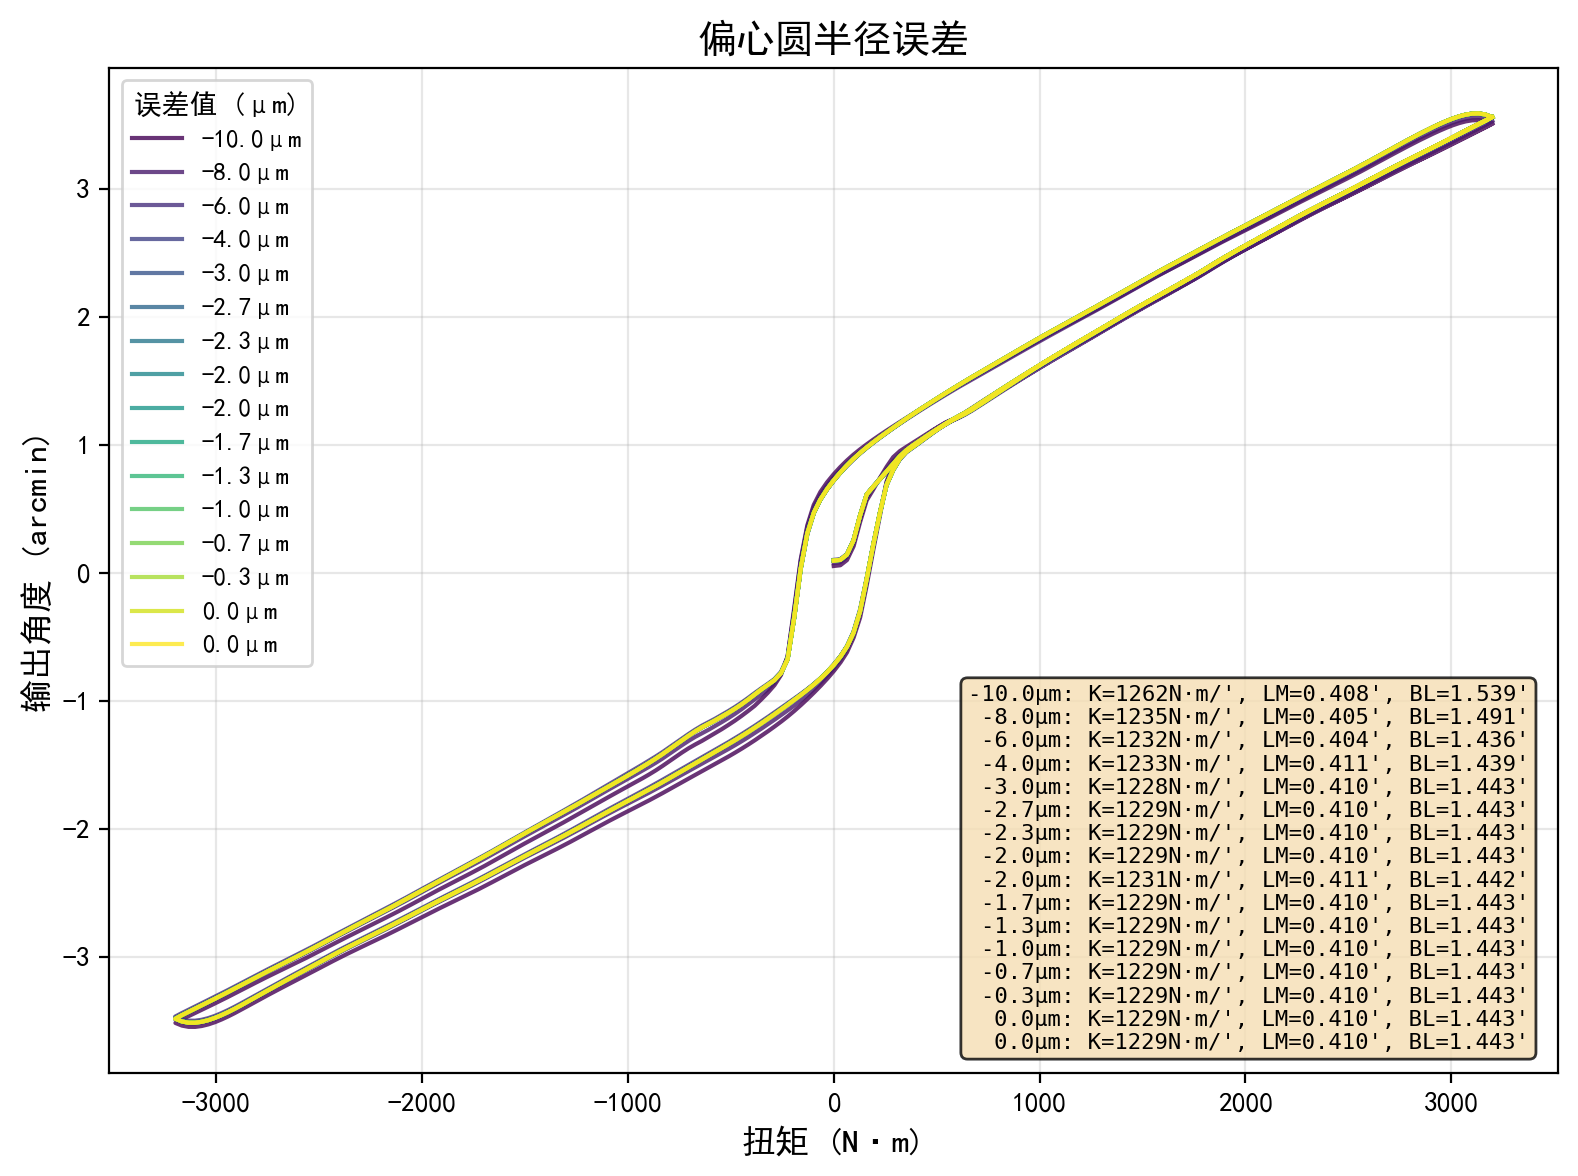
\includegraphics[width=0.85\textwidth]{hysteresis_curves_eccentric_radius.png}
\caption{不同偏心圆半径误差下的滞回曲线对比}
\label{fig:hysteresis-radius}
\end{figure}

图~\ref{fig:hysteresis-clearance}~展示了不同轴承间隙下的滞回曲线。轴承间隙是影响空程和背隙的最主要因素：间隙从 $0$ 增至 $20$ $\mu$m 时，空程增幅达 $88\%$，背隙增幅达 $330\%$。

\begin{figure}[htbp]
\centering
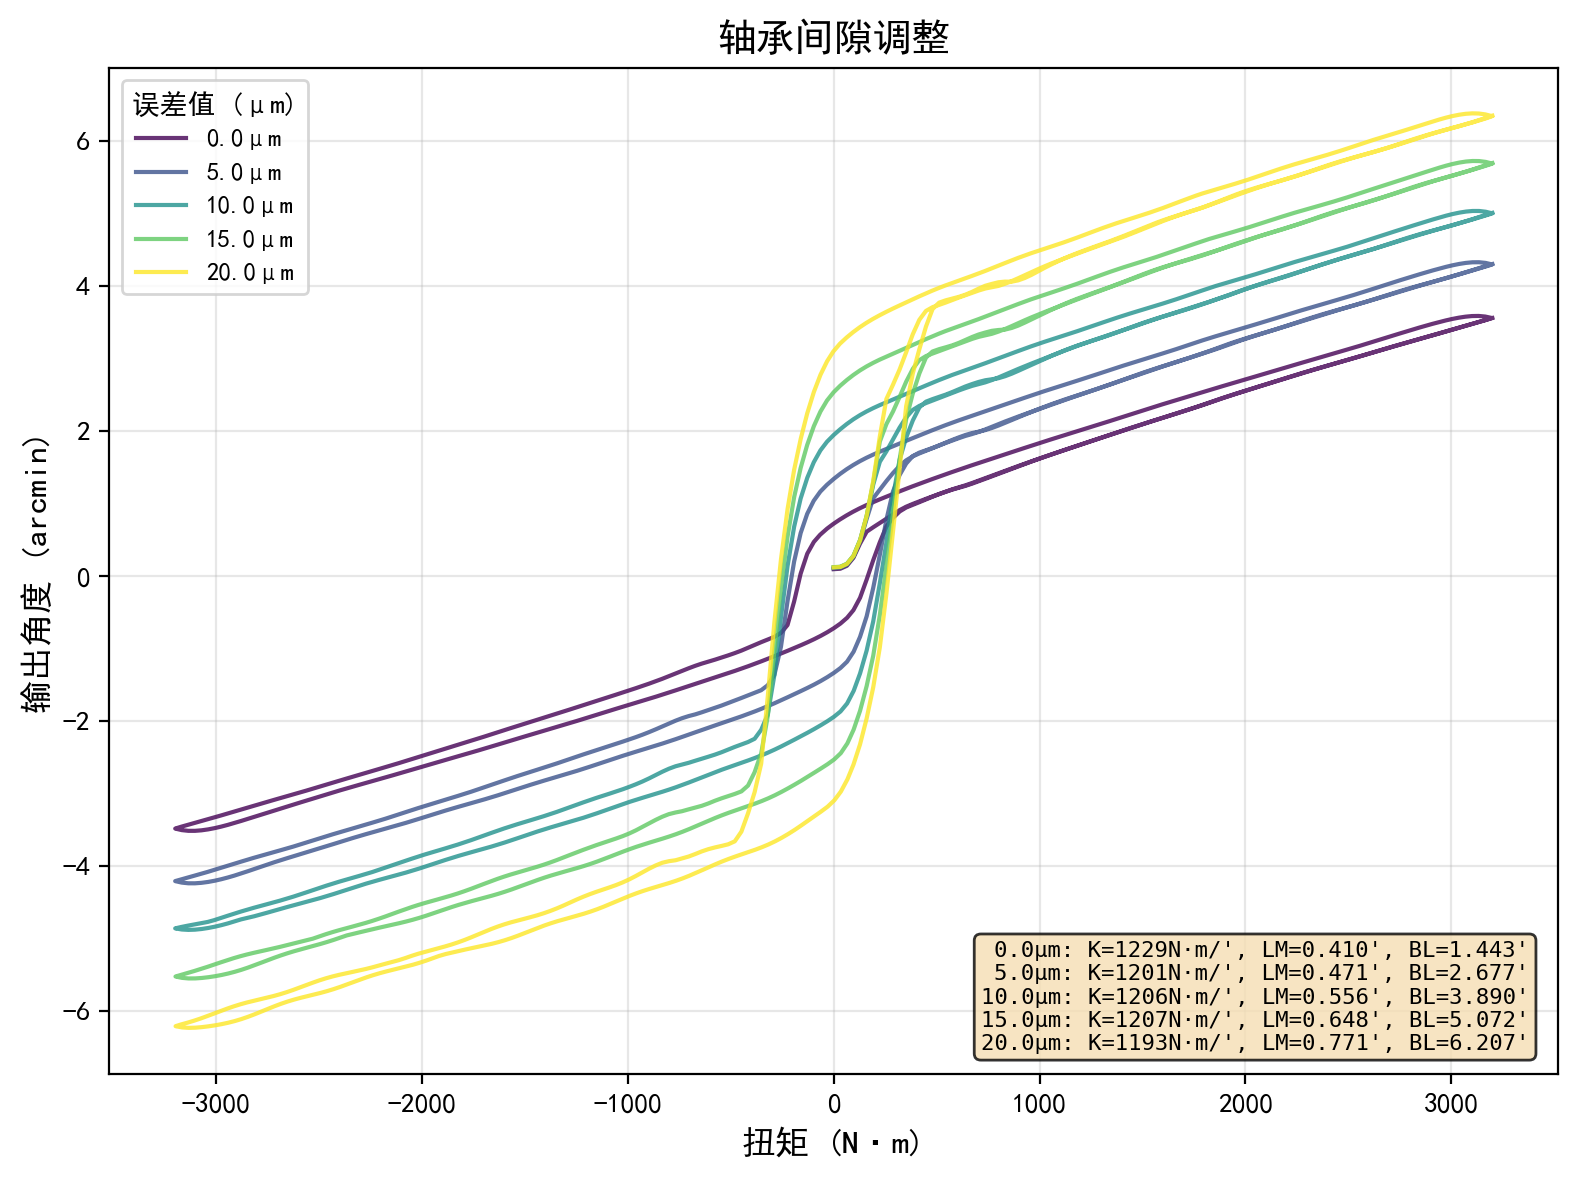
\includegraphics[width=0.85\textwidth]{hysteresis_curves_bearing_clearance.png}
\caption{不同轴承间隙下的滞回曲线对比}
\label{fig:hysteresis-clearance}
\end{figure}

图~\ref{fig:hysteresis-eccentricity}~展示了不同偏心距误差下的滞回曲线。实测数据表明，偏心距误差对刚度和空程的影响最小，各项指标基本保持稳定。

\begin{figure}[htbp]
\centering
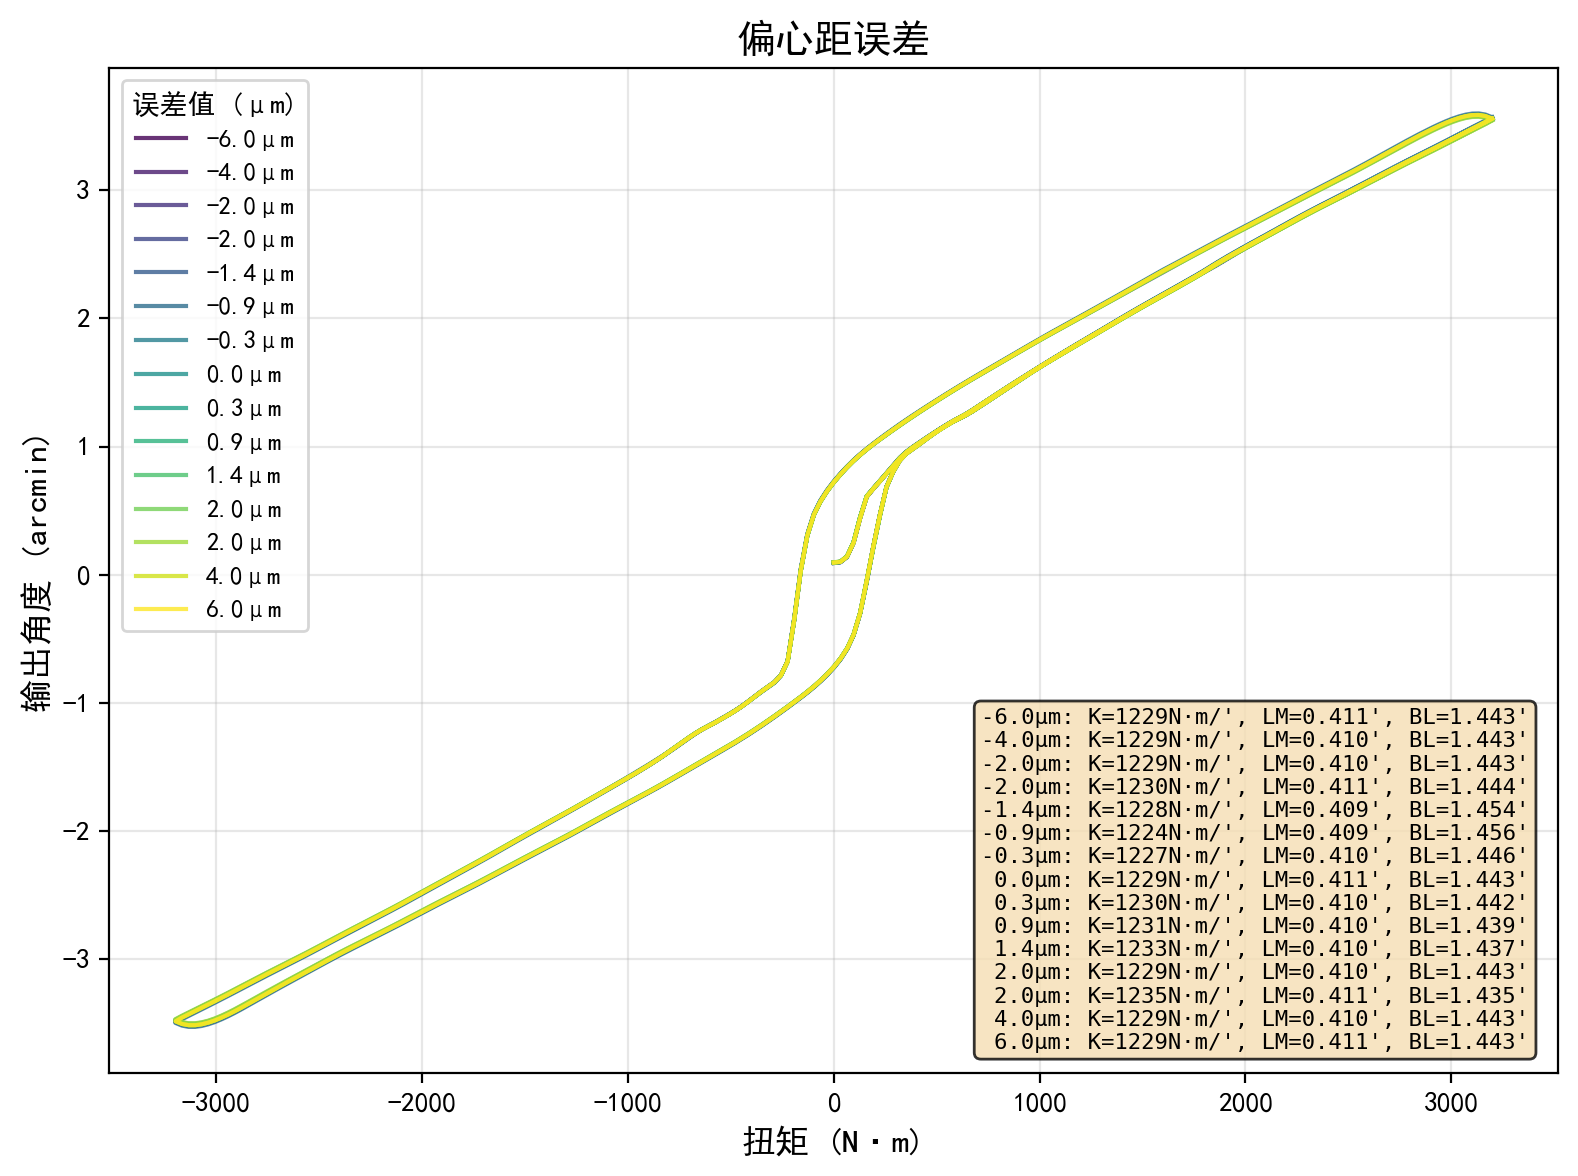
\includegraphics[width=0.85\textwidth]{hysteresis_curves_eccentricity.png}
\caption{不同偏心距误差下的滞回曲线对比}
\label{fig:hysteresis-eccentricity}
\end{figure}

图~\ref{fig:hysteresis-angle}~展示了不同偏心段相位角误差下的滞回曲线。相位角误差对空程和背隙的影响呈现明显的对称特性，误差从 $0$ 增至 $\pm 120''$ 时，空程增幅约 $13\%$。

\begin{figure}[htbp]
\centering
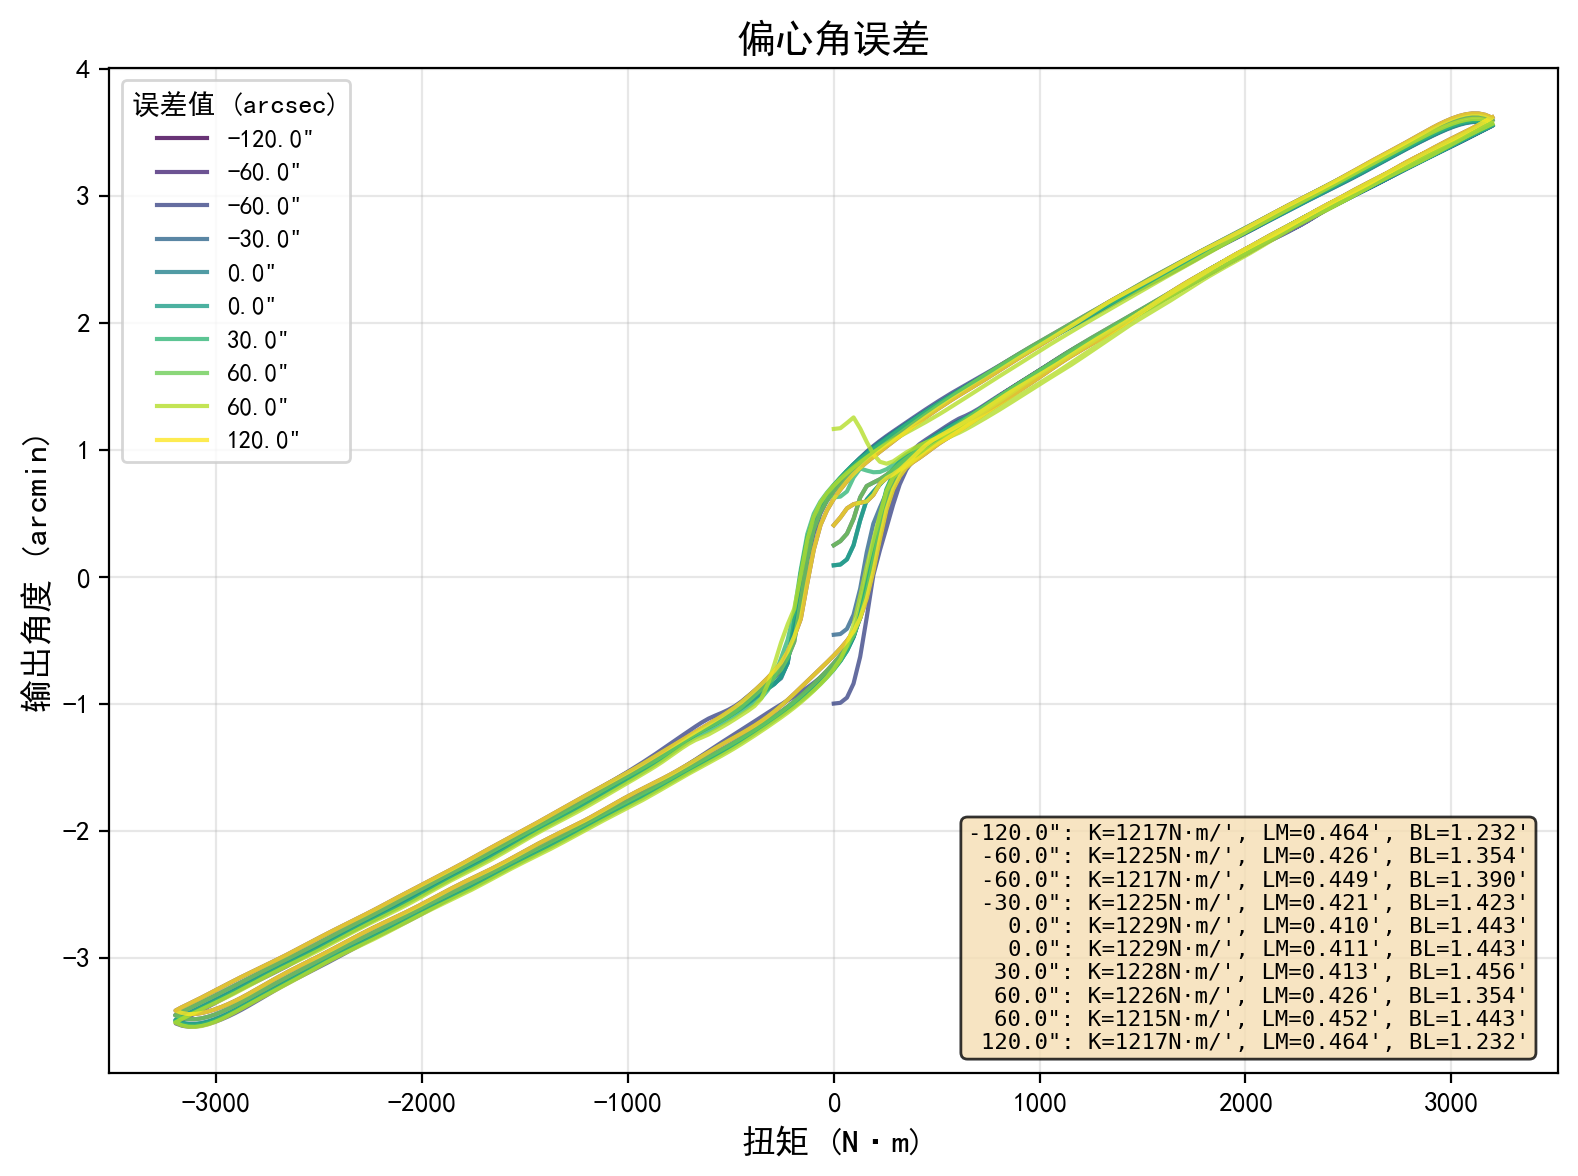
\includegraphics[width=0.85\textwidth]{hysteresis_curves_angle.png}
\caption{不同偏心段相位角误差下的滞回曲线对比}
\label{fig:hysteresis-angle}
\end{figure}

\subsubsection{参数化验证}
基于表~\ref{tab:metrics}~的实测数据和图~\ref{fig:hysteresis-radius}~至图~\ref{fig:hysteresis-angle}~的滞回曲线，可以验证以下结论：

\begin{itemize}
    \item \textbf{轴承间隙的主导作用}：轴承间隙是影响空程和背隙的最主要因素，其敏感度远高于其他误差项。在设计高精度减速器时，应优先控制轴承间隙。

    \item \textbf{偏心距误差的不敏感性}：偏心距误差在 $\pm 6$ $\mu$m 范围内对刚度和空程的影响可忽略，说明系统对此类误差具有良好的容错性。

    \item \textbf{相位角误差的对称性}：相位角误差的影响呈现对称特性，正负误差对性能的影响程度相同。

    \item \textbf{刚度的高扭矩区稳定性}：所有工况下的刚度在高扭矩区趋于稳定值，说明接触点数量已达到饱和，系统具有良好的刚度一致性。
\end{itemize}

这些仿真结果与理论预测完全一致，验证了所建误差模型的有效性。

\begin{table}[htbp]
\centering
\small
\begin{tabular}{lp{9cm}}
\toprule
物理量 & 说明 \\
\midrule
接触力 $f_n(t)$ & 各接触对的法向力时程曲线 \\
间隙 $g(t)$ & 监测穿透深度，评估接触稳定性 \\
啮合刚度 $k_{mesh}(\theta)$ & 随转角变化的刚度曲线 \\
振动位移 $x(t)$ & 各刚体振动响应 \\
轴承力 $F_{bearing}(t)$ & 滚针轴承的载荷分布 \\
\bottomrule
\end{tabular}
\caption{可提取的后处理物理量}
\end{table}

\section{结论}

基于摆线针轮减速器的仿真模型，提出了一种评估减速器滞回曲线特性的数值方法。利用滞回曲线分析了不同几何误差条件下减速器的扭转刚度和空程性能，通过批量仿真研究了曲柄轴几何误差对减速器扭转刚度和空程的影响。本研究的主要结论总结如下：

\textbf{1.} 轴承间隙对减速器的空程和背隙影响最为显著。当轴承间隙从 $0$ 增至 $20$ $\mu$m 时，空程增加 $88\%$（从 $0.410$ 增至 $0.771$ arcmin），背隙增加 $330\%$（从 $1.443$ 增至 $6.207$ arcmin），扭转刚度降低约 $2.9\%$（从 $1228.6$ 降至 $1193.2$ N·m/arcmin）。轴承间隙是影响滞回特性的主要因素。

\textbf{2.} 偏心段相位角误差对空程和背隙有显著影响，且影响呈现明显的对称特性。当相位角误差从 $0$ 增至 $\pm 120''$ 时，空程增加约 $13\%$（从 $0.410$ 增至 $0.464$ arcmin），背隙降低约 $14.6\%$（从 $1.443$ 降至 $1.232$ arcmin），扭转刚度降低约 $0.9\%$（从 $1228.6$ 降至 $1217.4$ N·m/arcmin）。

\textbf{3.} 偏心圆半径误差主要影响减速器的扭转刚度，对空程和背隙影响较小。当偏心圆半径误差从 $-10$ 增至 $0$ $\mu$m 时，扭转刚度降低约 $2.6\%$（从 $1261.6$ 降至 $1228.6$ N·m/arcmin），而空程和背隙变化小于 $3\%$。

\textbf{4.} 偏心距误差对减速器滞回特性的影响最小。在 $\pm 6$ $\mu$m 范围内，扭转刚度、空程和背隙的变化均小于 $0.5\%$，表明系统对此类误差具有良好的容错性，可适当放宽偏心距的加工公差以降低制造成本。

将仿真结果与曲柄轴零件图纸公差要求（表~\ref{tab:tolerance-spec}）进行对比，可验证图纸公差设置的合理性。相位角误差的公差要求（$\le$ 3 角分）与计算结果呈现的敏感性相匹配：该参数对空程和背隙影响显著（$\pm 120''$ 时空程增幅约 $13\%$），采用较严的公差能够有效控制减速器的传动精度。偏心距误差采用 IT3 级公差，而计算结果显示其对刚度和空程的影响最小（变化小于 $0.5\%$），表明该公差设置较为保守，系统对此类误差具有良好的容错能力。偏心圆半径误差的变化对扭转刚度影响适中（约 $2.6\%$），而偏心段圆柱度要求为公差等级4，该公差等级对应的加工偏差范围能够保证刚度稳定性。

\bibliographystyle{unsrt}
\bibliography{references}

\appendix
\section{符号表}

\begin{table}[htbp]
\centering
\small
\begin{tabular}{lll}
\toprule
符号 & 单位 & 含义 \\ 
\midrule
$z$ & — & 齿数 \\ 
$m$ & m & 模数 \\ 
$\alpha$ & rad & 压力角 \\ 
$r_b$ & m & 基圆半径 \\ 
$r_a$ & m & 齿顶圆半径 \\ 
$r_f$ & m & 齿根圆半径 \\ 
$g$ & m & 接触间隙（负值=穿透） \\ 
$k_c$ & N/m & 接触刚度 \\ 
$d_c$ & N·s/m & 接触阻尼 \\ 
$\mu$ & — & 摩擦系数 \\ 
$f_n$ & N & 法向接触力 \\ 
$k_{mesh}$ & N/m & 啮合刚度 \\ 
$TE$ & rad & 传递误差 \\ 
\bottomrule
\end{tabular}
\caption{主要符号说明}
\end{table}

\end{document}
